%%%%%%%%%%%%%%%%%%%%%%%%%%%%%%%%%%%%%%%%%%%%%%%%%
% ce-testsuite.tex
% 
% DESC: Latex source to be converted to HTML by tex4ht
%
%%%%%%%%%%%%%%%%%%%%%%%%%%%%%%%%%%%%%%%%%%%%%%%%%
\documentclass{article}

%%%%%%%%%%%%%%%%%%%%%%%%%%%%%%%%%%%%%%%%%%%%%%%%%
% PREAMBLE
%%%%%%%%%%%%%%%%%%%%%%%%%%%%%%%%%%%%%%%%%%%%%%%%%
\usepackage{hyperref}
\usepackage{listings}
\usepackage{color}
\usepackage[dvipsnames]{xcolor}
\usepackage{float}
\usepackage{graphicx}
\usepackage{tikz,tikz-dependency}

\usetikzlibrary{automata,positioning,external,shapes,arrows,chains,matrix,scopes,backgrounds}
% The following is for tikz externalization configuration which allows
% tikZ diagrams to render correctly while being processed by htlatex 
% http://tex.stackexchange.com/questions/158551/using-htlatex-with-tikz-dependency#158921
%%%%%%%%%%%%%%%%%%%%%%%%%%%%%%%%%%%%%%%%%%%%%%%%%
\tikzset{
    tex4ht inc/.style={
        /pgf/images/include external/.code={%
            \includegraphics[]{##1.svg}%
        }

    }
}
\tikzset{
 external/system call/.add={}                                                
      ; inkscape -z -f "\image.pdf" -l "\image.svg"
}
\makeatletter
\@ifpackageloaded{tex4ht}{
    \tikzexternalize[mode=only graphics]
}{
    \tikzexternalize
}
\makeatother

% Removes section numbers
\makeatletter
\renewcommand\thesection{}
%\renewcommand\thesubsection{\@arabic\c@section.\@arabic\c@subsection}
\renewcommand\thesubsection{}
\makeatother

% lstlisting configs for code syntax formatting
\lstdefinestyle{Java} {
  frame=tb,
  language=Java,
  aboveskip=3mm,
  belowskip=3mm,
  showstringspaces=false,
  columns=flexible,
  basicstyle={\large\ttfamily},
  numbers=none,
  numberstyle=\textcolor{gray},
  keywordstyle=\textcolor{red!75},
  commentstyle=\textcolor{dkgreen},
  stringstyle=\textcolor{blue},
  moredelim=[is][\textcolor{black!75}]{|}{|},
  breaklines=false,
  breakatwhitespace=true,
  tabsize=3
}
%%%%%%%%%%%%%%%%%%%%%%%%%%%%%%%%%%%%%%%%%%%%%%%%%
% COLOR DEFINITIONS
%%%%%%%%%%%%%%%%%%%%%%%%%%%%%%%%%%%%%%%%%%%%%%%%%
\tikzstyle{red}=[fill=red!30!white]
\tikzstyle{orange}=[fill=orange!30!white]
\tikzstyle{yellow}=[fill=yellow!30!white]
\tikzstyle{green}=[fill=green!30!white]
\tikzstyle{blue}=[fill=blue!30!white]
\tikzstyle{teal}=[fill=teal!30!white]
\tikzstyle{purple}=[fill=purple!30!white]
\tikzstyle{magenta}=[fill=magenta!30!white]
\tikzstyle{gray}=[fill=gray!30!white]
\tikzstyle{black}=[fill=black!30!white]

%%%%%%%%%%%%%%%%%%%%%%%%%%%%%%%%%%%%%%%%%%%%%%%%%
% DEFINE STACK COLORS
%%%%%%%%%%%%%%%%%%%%%%%%%%%%%%%%%%%%%%%%%%%%%%%%%
\definecolor{DEFINE_USR_COLOR}{HTML}{006699}
\definecolor{DEFINE_KRN_COLOR}{HTML}{003366}
\definecolor{DEFINE_HW_COLOR}{HTML}{000033}
\definecolor{DEFINE_CET_COLOR}{HTML}{339999}  
        
\tikzstyle{DK_COLOR}=[fill=blue!30!white]
\tikzstyle{ARQ_COLOR}=[fill=gray!30!white]
\tikzstyle{OS_COLOR}=[fill=black!50!white]
\tikzstyle{USR_COLOR}=[fill=DEFINE_USR_COLOR]
\tikzstyle{KRN_COLOR}=[fill=DEFINE_KRN_COLOR]
\tikzstyle{HW_COLOR}=[fill=DEFINE_HW_COLOR]
\tikzstyle{CET_COLOR}=[fill=DEFINE_CET_COLOR]
\tikzstyle{HM_COLOR}=[fill=cyan!30!white]
%%%%%%%%%%%%%%%%%%%%%%%%%%%%%%%%%%%%%%%%%%%%%%%%%
% STACK DIAGRAM DEFINITIONS
%%%%%%%%%%%%%%%%%%%%%%%%%%%%%%%%%%%%%%%%%%%%%%%%%
\tikzstyle{layer} = [rectangle, thick, rounded corners]
\tikzstyle{core_stack}= [layer, minimum width=11cm,minimum height=1cm, text = white]
\tikzstyle{user_stack}= [layer, minimum width=4cm,minimum height=1cm]
\tikzstyle{app_stack}=  [layer, minimum width=4.5cm,minimum height=3cm]
\tikzstyle{container}=  [layer, purple,minimum width=0.5cm,minimum height=0.5cm]

\tikzstyle{OS_LAYER} = [app_stack, OS_COLOR,fill=black!50!white, above left= 2.5cm and 0.1cm of USR.south, anchor=east, label={[label distance=-0.75cm]270:OpenShift}]
\tikzstyle{ARQ_LAYER} = [app_stack, ARQ_COLOR,label={[label distance=-0.75cm]270:Arquillian}, right= 0cm and 0.2cm of OS]
\tikzstyle{CET_LAYER} = [user_stack, CET_COLOR, above=of ARQ.south, anchor=south]
\tikzstyle{USR_LAYER} =  [core_stack, USR_COLOR, minimum height=4.5cm, label={[label distance=-0.75cm]270:\color{white}Userspace}]
\tikzstyle{KRN_LAYER} = [core_stack, KRN_COLOR, below= 0cm of USR]
\tikzstyle{HW_LAYER}  = [core_stack, HW_COLOR, below of=KRN]
\tikzstyle{DK_LAYER} = [user_stack, DK_COLOR]
\tikzstyle{HM_LAYER} = [user_stack, HM_COLOR]
%%%%%%%%%%%%%%%%%%%%%%%%%%%%%%%%%%%%%%%%%%%%%%%%%
% DOCUMENT
%%%%%%%%%%%%%%%%%%%%%%%%%%%%%%%%%%%%%%%%%%%%%%%%%
\iffalse
I don't want this to happen
\fi

\begin{document}

\centerline{\sc \large Cloud Enablement Test Suite}
\centerline{\sc Architecture for the Layperson }
\centerline{\url{https://github.com/jboss-openshift/ce-testsuite.git/}}

\vspace{1pc}
%================================================
% OVERVIEW
%================================================
\section{Overview}

\hspace{3pc} Leveraging container technology, Red Hat's Cloud Enablment(CE) team has developed a test suite to accelerate and stabilize the development of its middleware products. It is now far easier than before to create, test, and deploy middleware applications on the cloud. To harness the full power of this test suite, users should understand its architecture. This document serves as a basic overview of that architecture and its underlying mechanics.


%%%%%%%%%%%%%%%%%%%%%%%%%%%%%%%%%%%%%%%%%%%%%%%%%
% DIAGRAM OF PLATFORM ARCHITECTURE
%%%%%%%%%%%%%%%%%%%%%%%%%%%%%%%%%%%%%%%%%%%%%%%%%
\begin{figure}
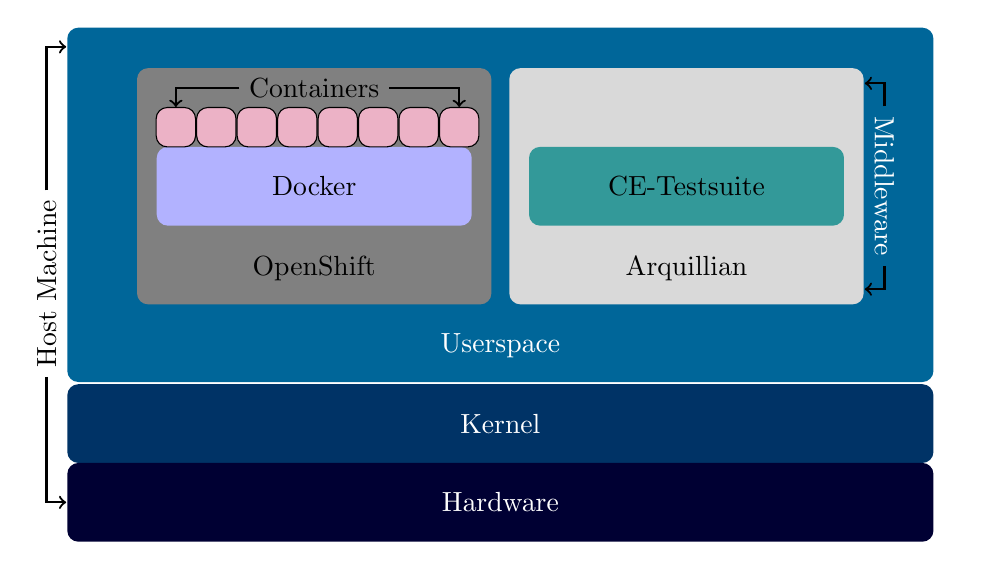
\begin{tikzpicture}[node distance = 1cm and 0cm]
      \tikzstyle{c}=  [container, draw=black, thin]
   
      %%%%%%%%%%%%%%%%%%%%%%%%%%%%%%%%%%%%%%%%%%%%%%%%%
      % LAYERS
      %%%%%%%%%%%%%%%%%%%%%%%%%%%%%%%%%%%%%%%%%%%%%%%%%
      \node[USR_LAYER] (USR) {};
      \node[OS_LAYER]  (OS)  {};
      \node[ARQ_LAYER] (ARQ) {};
      \node[CET_LAYER] (CET) {CE-Testsuite};
      \node[KRN_LAYER] (KRN) {Kernel};
      \node[HW_LAYER]  (HW)  {Hardware};
      
      %%%%%%%%%%%%%%%%%%%%%%%%%%%%%%%%%%%%%%%%%%%%%%%%%
      % DOCKER + CONTAINERS
      %%%%%%%%%%%%%%%%%%%%%%%%%%%%%%%%%%%%%%%%%%%%%%%%%
      \node[user_stack, DK_COLOR, above=of OS.south, anchor=south ] (DK) {Docker};
      \node[c, above= 0.75cm of DK.west, anchor=west ] (C1) {};
      \node[c, right= of C1] (C2) {};
      \node[c, right= of C2] (C3) {};
      \node[c, right= of C3] (C4) {};
      \node[c, right= of C4] (C5) {};  
      \node[c, right= of C5] (C6) {};
      \node[c, right= of C6] (C7) {};
      \node[c, right= of C7] (C8) {};
      
      %%%%%%%%%%%%%%%%%%%%%%%%%%%%%%%%%%%%%%%%%%%%%%%%%
      % LABELS AND ARROWS
      %%%%%%%%%%%%%%%%%%%%%%%%%%%%%%%%%%%%%%%%%%%%%%%%%
      \node [above= of DK.center] (C) {Containers};
      \path[->,thick, to path={-| (\tikztotarget)}] 
      (C.west) edge (C1.north)
      (C.east) edge (C8.north);
                 
      \node [rotate=90, below left= 1cm and .25cm of USR.west, anchor=center] (HM) {Host Machine};
      \path[->, thick, to path={|- (\tikztotarget)}] 
      (HM.east) edge (USR.160)
      (HM.west) edge (HW.180);
        
      \node [rotate=90, below right= 1cm and .25cm of USR.east, anchor=center] (BLANK) {};
       
      \node [right= 0cm and .25cm of ARQ.east, anchor=center, rotate=270] (MW) {\color{white}Middleware};
      \path[->, thick, to path={|- (\tikztotarget)}] 
      (MW.west) edge (ARQ.30)
      (MW.east) edge (ARQ.330);
      
\end{tikzpicture}
\caption{Diagram of Platform Architecture} 
\end{figure}

%================================================
% CONTAINER TECHNOLOGY
%================================================
\section{Container technology}
%\hspace{3pc} 
In order for applications to run on cloud platforms such as OpenShift, they must be "containerized". Moreover, these applications must be rewritten, generated, or transported into
isolated programming environments known as containers. 
%================================================
% CONTAINERS
%================================================
\subsection{Containers}

%\hspace{3pc}
A container is essentially an isolated userspace containing its own read/write filesystem, processes, network ports, and libraries. By relying on the functionality of their host's kernel, containers save on resource costs, earning the trait of being "lightweight". With little expense, containers can be instantiated, snapshotted, and destroyed quickly. Moreover, containers are ideal for developing applications. By providing applications with their own isolated programming environment, containers help users avoid problems like dependency and networking collisions. Accidentally downloading conflicting libraries or necromancing zombie network ports need not result in tedious environment debugging when developing in a container. Remember, containers are inexpensive, they can be destroyed and then recreated on a whim. 

%%%%%%%%%%%%%%%%%%%%%%%%%%%%%%%%%%%%%%%%%%%%%%%%%
% CONTAINER DIAGRAM
%%%%%%%%%%%%%%%%%%%%%%%%%%%%%%%%%%%%%%%%%%%%%%%%%
\begin{figure}
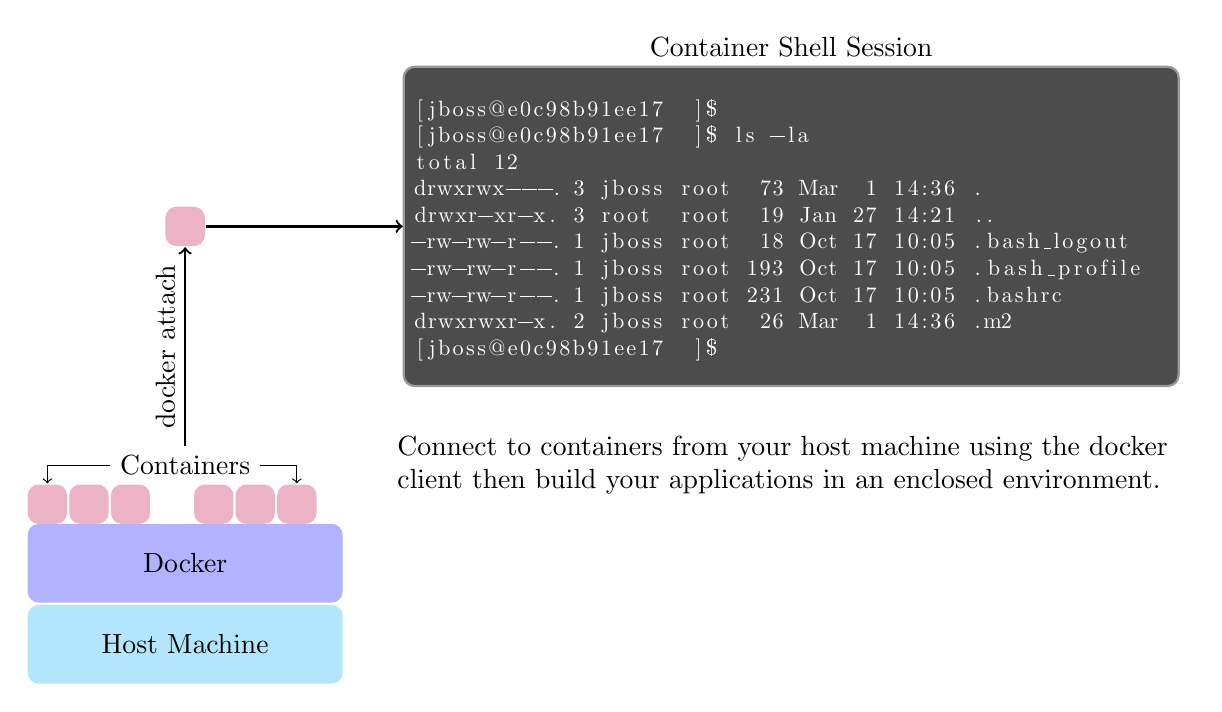
\begin{tikzpicture}[node distance = 1cm and 0cm]
      \tikzstyle{big_container}=[container, minimum width=0.5cm,minimum height=0.5cm]
      \tikzstyle{shell}=[layer, minimum width=5.0cm,minimum height=2.0cm,text width=4cm,draw=gray!80, fill=black!70!white,text=white, text width=12cm, scale=.8, inner sep=1ex]
      
      %%%%%%%%%%%%%%%%%%%%%%%%%%%%%%%%%%%%%%%%%%%%%%%%%
      % DOCKER + CONTAINERS
      %%%%%%%%%%%%%%%%%%%%%%%%%%%%%%%%%%%%%%%%%%%%%%%%%
      \node[user_stack, DK_COLOR] (DK) {Docker};
      \node[container, above= 0.75cm of DK.west, anchor=west ] (C1) {};
      \node[container, right= of C1] (C2) {};
      \node[container, right= of C2] (C3) {};
      \node[container, fill=white, right= of C3] (C4) {};
      \node[container, right= of C4] (C5) {};  
      \node[container, right= of C5] (C6) {};
      \node[container, right= of C6] (C7) {};
      
      \node[user_stack, fill=cyan!30!white, below=0cm of DK] (HM) {Host Machine};
      %%%%%%%%%%%%%%%%%%%%%%%%%%%%%%%%%%%%%%%%%%
      % CONTAINER SQUARE
      %%%%%%%%%%%%%%%%%%%%%%%%%%%%%%%%%%%%%%%%%%
      \node[big_container, above= 3.5cm of DK.north, anchor=south] (BIG_CONTAINER) {};
      %%%%%%%%%%%%%%%%%%%%%%%%%%%%%%%%%%%%%%%%%%
      % SHELL
      %%%%%%%%%%%%%%%%%%%%%%%%%%%%%%%%%%%%%%%%%%%
      \node[shell,right= 2.5cm of BIG_CONTAINER] (C_SHELL){
      \begin{lstlisting}
[jboss@e0c98b91ee17  ]$
[jboss@e0c98b91ee17  ]$ ls -la
total 12
drwxrwx---. 3 jboss root  73 Mar  1 14:36 .
drwxr-xr-x. 3 root  root  19 Jan 27 14:21 ..
-rw-rw-r--. 1 jboss root  18 Oct 17 10:05 .bash_logout
-rw-rw-r--. 1 jboss root 193 Oct 17 10:05 .bash_profile
-rw-rw-r--. 1 jboss root 231 Oct 17 10:05 .bashrc
drwxrwxr-x. 2 jboss root  26 Mar  1 14:36 .m2
[jboss@e0c98b91ee17  ]$
      \end{lstlisting} };
      
      %%%%%%%%%%%%%%%%%%%%%%%%%%%%%%%%%%%%%%%%%%%%%%%%%
      % LABELS AND ARROWS
      %%%%%%%%%%%%%%%%%%%%%%%%%%%%%%%%%%%%%%%%%%%%%%%%%
      \node [align=left, text width=10.0cm,below= 0.5cm of C_SHELL.south] (SHELL_DESC) {Connect to containers from your host machine using the docker client then build your applications in an enclosed environment.};
      \node [above= of DK.center] (C) {Containers};
      \path[->, to path={-| (\tikztotarget)}] 
      (C.west) edge (C1.north)
      (C.east) edge (C7.north);
      \node[above=0cm and 0cm of C_SHELL] (SHELL_LABEL) {Container Shell Session};
      %%%%%%%%%%%%%%%%%%%%%%%%%%%%%%%%%%%%%%%%%%
      % PATHS
      %%%%%%%%%%%%%%%%%%%%%%%%%%%%%%%%%%%%%%%%%%%
      \path[->, thick] (BIG_CONTAINER) edge (C_SHELL);
      \draw[->, thick] (C) -- node [above, rotate=90] {docker attach} (BIG_CONTAINER);
\end{tikzpicture}
\caption{Connecting to Containers from Host Machine} 
\end{figure}

\subsection{Container Management}
One can manage these userspaces using the container interface application known as Docker. Docker uses features built in the kernel to organize, isolate, create, save, and destroy containers. Friends running Docker on their machine can easily share their applications with other friends running Docker. These packaged applications not only deliver the same executing code of the developer but also the same environment that executing code was running in. All libraries and environmental variables are installed and ready to go. This way, more time can be spent creating the application as opposed to debugging environmental infestations.

\begin{figure}
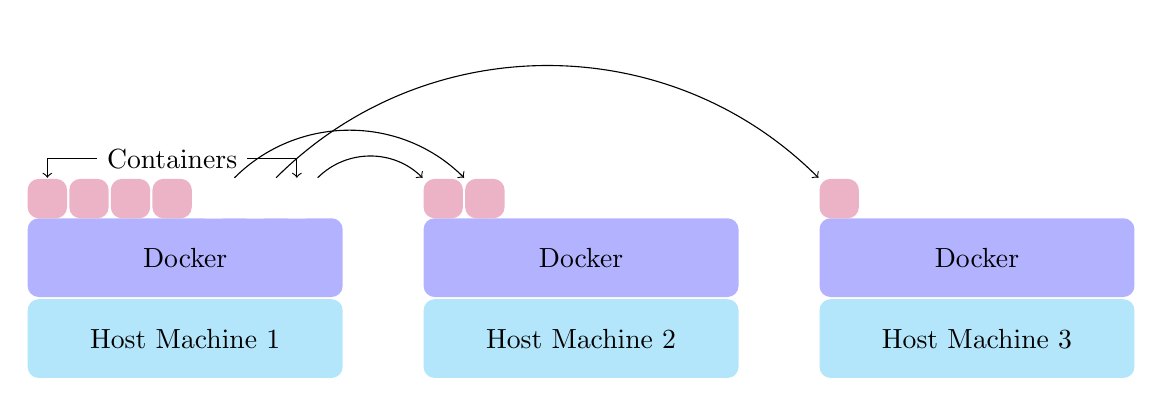
\begin{tikzpicture}[node distance = 1cm and 0cm]

      %%%%%%%%%%%%%%%%%%%%%%%%%%%%%%%%%%%%%%%%%%
      % HOST MACHINE 1
      %%%%%%%%%%%%%%%%%%%%%%%%%%%%%%%%%%%%%%%%%%%
      \node[DK_LAYER] (DK1) {Docker};
      \node[container, above= 0.75cm of DK1.west, anchor=west] (C1) {};
      \node[container, right= of C1]      (C2)        {};
      \node[container, right= of C2]      (C3)        {};
      \node[container, right= of C3]      (C4)        {};
      \node[container, fill=white, right= of C4]      (C5)        {};  
      \node[container, fill=white, right= of C5]      (C6)        {};
      \node[container, fill=white, right= of C6]      (C7)        {};
      \node[HM_LAYER, below=0cm of DK1] (HM1) {Host Machine 1};
       
      \node [above= 0cm and 0cm of C4] (C) {Containers};
      \path[->, to path={-| (\tikztotarget)}] 
      (C.west) edge (C1.north)
      (C.east) edge (C7.north);
      
      %%%%%%%%%%%%%%%%%%%%%%%%%%%%%%%%%%%%%%%%%%
      % HOST MACHINE 2
      %%%%%%%%%%%%%%%%%%%%%%%%%%%%%%%%%%%%%%%%%%%
      \node[DK_LAYER, right= 0cm and 1cm of DK1] (DK2) {Docker};
      \node[container, above= 0.75cm of DK2.west, anchor=west] (CR1) {};
      \node[HM_LAYER, below=0cm of DK2] (HM2) {Host Machine 2};
      
      %%%%%%%%%%%%%%%%%%%%%%%%%%%%%%%%%%%%%%%%%%
      % HOST MACHINE 3
      %%%%%%%%%%%%%%%%%%%%%%%%%%%%%%%%%%%%%%%%%%%
      \node[DK_LAYER, right=0cm and 1cm of DK2] (DK3) {Docker};
      \node[container, above= 0.75cm of DK3.west, anchor=west]  (CRR1) {};
      \node[container, right=of CR1] (CRR2) {};
      \node[HM_LAYER, below=0cm of DK3] (HM3) {Host Machine 3};
      
      \path[->, bend left=45] (C7) edge (CR1);
      \path[->, bend left=45] (C6) edge (CRR1);
      \path[->, bend left=45] (C5) edge (CRR2);
      
\end{tikzpicture}
\caption{Sharing Containers with Friends} 
\end{figure}
In contrast to virtual machines, containers are classified under operating system level virtualization because they rely on the operating system resources of their host machine. Virtual machines rely on hardware virtualization which has a higher virtual memory management cost than operating system virtualization. Intuitively, this makes sense. It is more expensive to replicate the hardware and operating system for a virtual machine than it is to instantiate an isolated userspace for a container. Although containers provide less isolation than virtual machines, they consume significantly less resources. This is why containers are viewed as being "light". In fact, it is even possible for a single physical machine to host hundreds containers simultaneously. %However, as one can imagine, this can become difficult to manage.

\noindent\makebox[\textwidth]{\rule{\textwidth}{7pt}} Work in Progress

%%%%%%%%%%%%%%%%%%%%%%%%%%%%%%%%%%%%%%%%%%%%%%%%%
% CONTAINER ORCHESTRATION
%%%%%%%%%%%%%%%%%%%%%%%%%%%%%%%%%%%%%%%%%%%%%%%%%
\subsection{Container Orchestration(WIP)}
%As a containerized application grows, it becomes complicated to manage. This is where applications like OpenShift come to play. They abstract the container world

%Managing containerized applications can get complicated when
%Openshift is an application which organizes and manages containers for application needs. The ability to generate containers in bulk has seduced some into creating applications that can scatter these multitudes of containers. Container platforms like OpenShift abstract the users away from where their apps may be running.   

%Distributed openshift and pod diagram
%%%%%%%%%%%%%%%%%%%%%%%%%%%%%%%%%%%%%%%%%%%%%%%%%
% OPENSHIFT PLATFORM
%%%%%%%%%%%%%%%%%%%%%%%%%%%%%%%%%%%%%%%%%%%%%%%%%
\begin{figure}
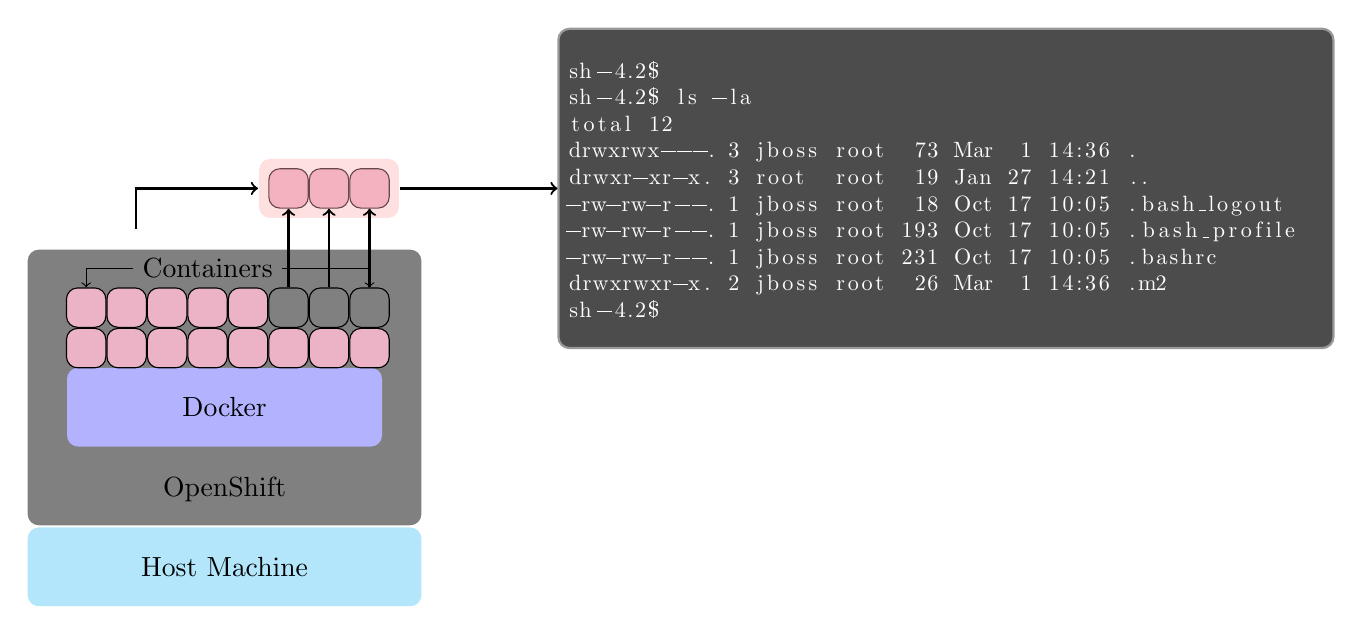
\begin{tikzpicture}[node distance = 1cm and 0cm]
      \tikzstyle{c}=  [container, draw=black, thin]
      \tikzstyle{shell}=[layer, minimum width=5.0cm,minimum height=2.0cm,text width=4cm,draw=gray!80, fill=black!70!white,text=white, text width=12cm, scale=.8, inner sep=1ex]
      
      \node[USR_LAYER, minimum width = 1cm, minimum height = 1cm] (USR)  {};
      
      \node[OS_LAYER, minimum width=5cm, minimum height = 3.5cm, below= 0cm and 0cm of USR.center, anchor=center] (OS) {};
      \node[DK_LAYER,  DK_COLOR, above=of OS.south, anchor=south] (DK)    {Docker};
      \node[c, above= 0.75cm of DK.west, anchor=west] (C1) {};
      \node[c, right= of C1]      (C2)        {};
      \node[c, right= of C2]      (C3)        {};
      \node[c, right= of C3]      (C4)        {};
      \node[c, right= of C4]      (C5)        {};  
      \node[c, right= of C5]      (C6)        {};
      \node[c, right= of C6]      (C7)        {};
      \node[c, right= of C7]      (C8)        {};
      
      \node[c, above= 0cm and 0cm of C1] (C21) {};
      \node[c, right= of C21] (C22) {};
      \node[c, right= of C22] (C23) {};
      \node[c, right= of C23] (C24) {};
      \node[c, right= of C24] (C25) {};  
      \node[c, OS_COLOR, right= of C25] (C26) {};
      \node[c, OS_COLOR, right= of C26] (C27) {};
      \node[c, OS_COLOR, right= of C27] (C28) {};
       
      \node [above= 0cm of C24 ] (C) {Containers};
      \path[->, to path={-| (\tikztotarget)}] 
      (C.west) edge (C21.north)
      (C.east) edge (C28.north);
      
      \node[HM_LAYER, minimum width = 5cm, below= 0cm of OS] (HM) {Host Machine};   
      
      \tikzstyle{c}=  [container, draw=black, thin]
      \tikzstyle{pod}=[thick, opacity=0.4, rounded corners]
             
      %%%%%%%%%%%%%%%%%%%%%%%%%%%%%%%%%%%%%%%%%%%%%%%%%
      % POD DIVISION
      %%%%%%%%%%%%%%%%%%%%%%%%%%%%%%%%%%%%%%%%%%%%%%%%%
      % pod
      \node[c, above= 1cm of C26]  (P1)        {};
      \node[c, right= of P1]      (P2)        {};
      \node[c, right= of P2]      (P3)        {};  
      \node[pod,fill=red!30!white, fit=(P1)(P2)(P3)] (pod) {};
      
      \path[->, thick] (C26) edge (P1);
      \path[->, thick] (C27) edge (P2);
      \path[->, thick] (C28) edge (P3);
      
      %%%%%%%%%%%%%%%%%%%%%%%%%%%%%%%%%%%%%%%%%%
      % SHELL
      %%%%%%%%%%%%%%%%%%%%%%%%%%%%%%%%%%%%%%%%%%%
      \node[shell,right= 2cm of pod] (P_SHELL){
      \begin{lstlisting}
sh-4.2$
sh-4.2$ ls -la
total 12
drwxrwx---. 3 jboss root  73 Mar  1 14:36 .
drwxr-xr-x. 3 root  root  19 Jan 27 14:21 ..
-rw-rw-r--. 1 jboss root  18 Oct 17 10:05 .bash_logout
-rw-rw-r--. 1 jboss root 193 Oct 17 10:05 .bash_profile
-rw-rw-r--. 1 jboss root 231 Oct 17 10:05 .bashrc
drwxrwxr-x. 2 jboss root  26 Mar  1 14:36 .m2
sh-4.2$
      \end{lstlisting} };
      
      \node [above left = 0cm and 1cm  of OS.north] (os1) {};
      \path[->, thick, rotate=90, to path={-| (\tikztotarget)}] 
      %(OS.north) edge (os1)
      (os1) edge node [above] {oc rsh} (pod);
      %(os1) edge (pod.west);
      
      %\draw[->, thick] (openshift) -- node [above, rotate=90] {oc rsh} (BIG_CONTAINER);
      \path[->, thick] (pod) edge (P_SHELL.west);
\end{tikzpicture}
\caption{OpenShift Platform}
\end{figure}

Openshift organizes containers into groups specific for applications. These groupings of containers are known as pods. Most of the operations which Openshift will preform are upon pods for easier management and groupings. A pod must have at least one container and pods are the smallest unit with which openShift can manipulate.
%A pod has its own ip address, containers in a pod can share storage and networking(owns port space) acts as a virtual operating system. pods are imutable, must update and restart config to make changes
%machine instance, virtual operating system
%%%%%%%%%%%%%%%%%%%%%%%%%%%%%%%%%%%%%%%%%%%%%%%%%
% OPENSHIFT APPLICATION STACK, Pod Division
%%%%%%%%%%%%%%%%%%%%%%%%%%%%%%%%%%%%%%%%%%%%%%%%%
\begin{figure}
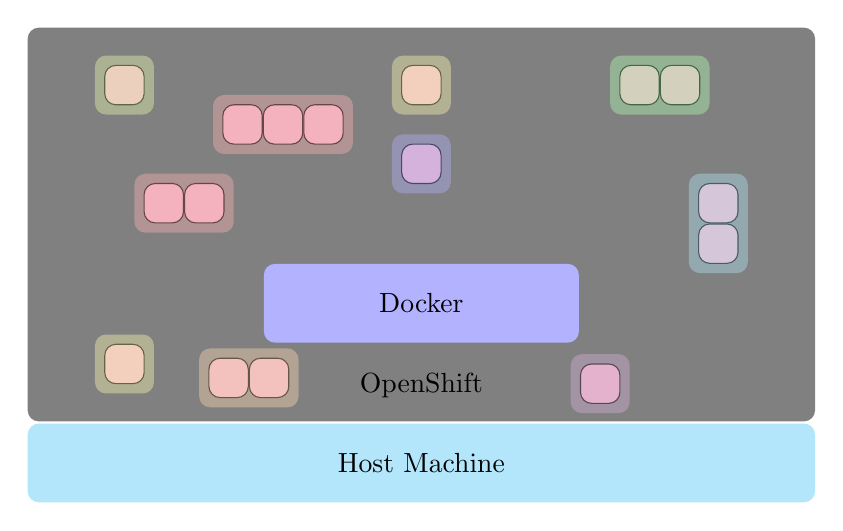
\begin{tikzpicture}[node distance = 1cm and 0cm]
      \tikzstyle{c}=  [container, draw=black, thin]
      \tikzstyle{pod}=[thick, opacity=0.4, rounded corners]
       
      \node[USR_LAYER, minimum width = 2cm] (USR)  {};
      
      \node[OS_LAYER, minimum width=10cm, minimum height = 5cm, below= 0cm and 0cm of USR.center, anchor=center] (OS) {};
      
      \node[DK_LAYER,  DK_COLOR, above=of OS.south, anchor=south] (DK)    {Docker};
      
      %%%%%%%%%%%%%%%%%%%%%%%%%%%%%%%%%%%%%%%%%%%%%%%%%
      % POD DIVISIONS
      %%%%%%%%%%%%%%%%%%%%%%%%%%%%%%%%%%%%%%%%%%%%%%%%%
      % pod1
      \node[c, above left= 2cm and 1.5cm of DK] (C1) {};
      \node[pod,fill=lime!30!white, fit=(C1)] (pod1) {};
       
      % pod2
      \node[c, above= 2cm of DK] (C27) {};
      \node[pod,fill=yellow!30!white, fit=(C27)] (pod2) {};
      
      % pod3
      \node[c, above left= 1.5cm and 0.0cm of DK]      (C3)        {};
      \node[c, right= of C3]      (C4)        {};
      \node[c, right= of C4]      (C5)        {};  
      \node[pod,fill=red!30!white, fit=(C3)(C4)(C5)] (pod3) {};
      
      % pod4
      \node[c, below left= 0.25cm of DK] (C31) {};
      \node[c, right= of C31] (C32) {};
      \node[pod,fill=orange!30!white, fit=(C31)(C32)] (pod4) {};
       
      % pod5
      \node[c, below left= 0cm and 1.5cm of DK] (C28) {};
      \node[pod,fill=yellow!30!white, fit=(C28)] (pod5) {};
       
      % pod6
      \node[c, above right= 0.5cm and 1.5cm of DK] (C21) {};
      \node[c, below= 0cm of C21] (C22) {};
      \node[pod,fill=cyan!30!white, fit=(C21)(C22)] (pod6) {};
      
      % pod7
      \node[c, below right= 0.25cm and 0cm of DK] (C6) {};
      \node[pod,fill=violet!30!white, fit=(C6)] (pod7) {};
    
      % pod8 
      \node[c, above= of DK]  (C33) {};
      \node[pod,fill=blue!30!white, fit=(C33)] (pod8) {};
       
      % pod9
      \node[c, above left= 0.5 cm and 1.0cm of DK] (C41) {};
      \node[c, right= of C41] (C42) {};
      \node[pod,fill=red!30!white, fit=(C41)(C42)] (pod9) {};
     
      % pod10
      \node[c, above right= 2cm and 0.5cm of DK] (C45) {};  
      \node[c, right= 0cm of C45]         (C46) {};
      \node[pod,fill=green!30!white, fit=(C45)(C46)] (pod10) {};
     
     
      \node[HM_LAYER, minimum width = 10cm, below= 0cm of OS] (HM) {Host Machine};    
\end{tikzpicture}
\caption{OpenShift Platform, Pod Division}
\end{figure}

Organize your pods into namespaces to help avoid appliction naming collisions by decreasing the scope of your applications
%%%%%%%%%%%%%%%%%%%%%%%%%%%%%%%%%%%%%%%%%%%%%%%%%
% OPENSHIFT APPLICATION STACK, NAMESPACE DIVISON
%%%%%%%%%%%%%%%%%%%%%%%%%%%%%%%%%%%%%%%%%%%%%%%%%
\begin{figure}
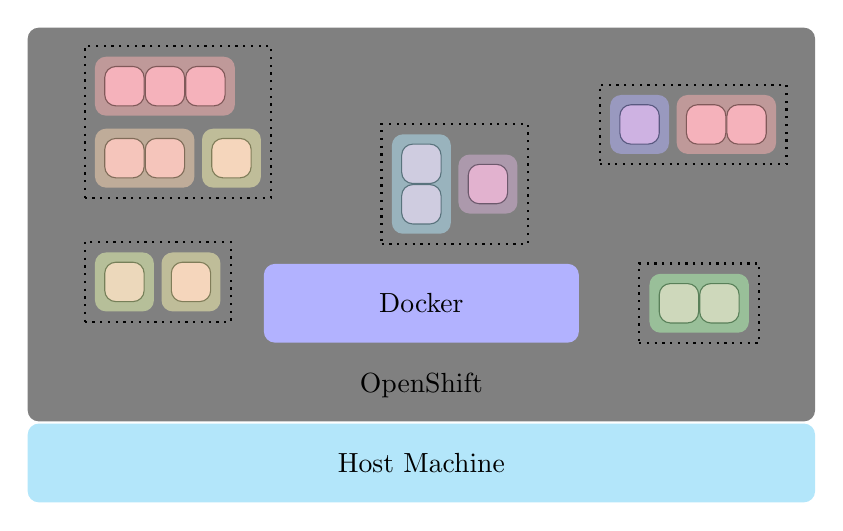
\begin{tikzpicture}[node distance = 1cm and 0cm]
      \tikzstyle{c}=  [container, draw=black, thin]
      \tikzstyle{pod}=[thick, opacity=0.5, rounded corners]
      \tikzstyle{NS}=[thick, draw, dotted] %Namespace
           
      \node[USR_LAYER, minimum width = 2cm] (USR)  {};
      
      \node[OS_LAYER, minimum width=10cm, minimum height = 5cm, below= 0cm and 0cm of USR.center, anchor=center] (OS) {};
      
      \node[DK_LAYER,  DK_COLOR, above=of OS.south, anchor=south] (DK)    {Docker};
      
      %%%%%%%%%%%%%%%%%%%%%%%%%%%%%%%%%%%%%%%%%%%%%%%%%
      % NAMESPACE DIVISIONS
      %%%%%%%%%%%%%%%%%%%%%%%%%%%%%%%%%%%%%%%%%%%%%%%%%
      % NS1
      \node[c, above left= -0.5cm and 1.5cm of DK] (C1) {};
      \node[pod,fill=lime!30!white, fit=(C1)] (pod1) {};
      \node[c, right= 0cm and 0.2cm of pod1] (C27) {};
      \node[pod,fill=yellow!30!white, fit=(C27)] (pod2) {};
      \node[NS, fit=(pod1)(pod2)] (NS1) {};
      
      % NS2
      \node[c, above left= 2.5cm and 1.5cm of DK.west] (C3) {};
      \node[c, right= of C3]      (C4)        {};
      \node[c, right= of C4]      (C5)        {};  
      \node[pod,fill=red!30!white, fit=(C3)(C4)(C5)] (pod3) {};
      
      \node[c, below= 0.4cm of C3] (C31) {};
      \node[c, right= of C31] (C32) {};
      \node[pod,fill=orange!30!white, fit=(C31)(C32)] (pod4) {};
      
      \node[c, right= 0cm and 0.2cm of pod4] (C28) {};
      \node[pod,fill=yellow!30!white, fit=(C28)] (pod5) {};
      
      \node[NS, fit=(pod3)(pod4)(pod5)] (NS2) {};
      
      %NS3
      \node[c, above= of DK]     (C21) {};
      \node[c, below= 0cm of C21] (C22) {};
      \node[pod, fill=cyan!30!white, fit=(C21)(C22)] (pod6) {};
           
      \node[c, right= 0cm and 0.2cm of pod6] (C6) {};
      \node[pod,fill=violet!30!white, fit=(C6)] (pod7) {};
      
      \node[NS, fit=(pod6)(pod7)] (NS3) {};
        
      %NS4
      \node[c, above right= 1.5cm and 0.5 of DK]  (C33) {};
      \node[pod,fill=blue!30!white, fit=(C33)] (pod8) {};
 
      \node[c, right=0cm and 0.2cm of pod8] (C41) {};
      \node[c, right= of C41] (C42) {};
      \node[pod,fill=red!30!white, fit=(C41)(C42)] (pod9) {};
      
      \node[NS, fit=(pod8)(pod9)] (NS4) {};
     
      %NS5
      \node[c, right= 0cm and 1cm of DK.east] (C45) {};  
      \node[c, right= 0cm of C45]         (C46) {};
      \node[pod,fill=green!30!white, fit=(C45)(C46)] (pod10) {};
      \node[NS, fit=(pod10)] (NS7) {};
     
      \node[HM_LAYER, minimum width = 10cm, below= 0cm of OS] (HM) {Host Machine}; 
    
\end{tikzpicture}
\caption{OpenShift Platform, Namespace Division}
\end{figure}
%================================================
% CONTAINERS
%================================================
\subsection{Container Testing(WIP)}



%================================================
% CONTAINER TECHNOLOGY
%================================================
\section{Middleware(WIP)}

%\noindent Currently, the Cloud Enablement team is dockerizing several Red Hat middleware products:
%\begin{itemize}
%\item AMQ(Advanced Message Queuing)
%\item EAP(Enterprise Application Platform)
%\item JDG(JBoss Data Grid)
%\item Kieserver(Realtime Decision Server)
%\item Spark(Cluster Computing Framework)
%\item SSO(Single Sign-on)
%\item Tomcat(JBoss Webserver)
%\end{itemize} 
%\noindent 
%

\iffalse
I don't want this to happen
\begin{figure}
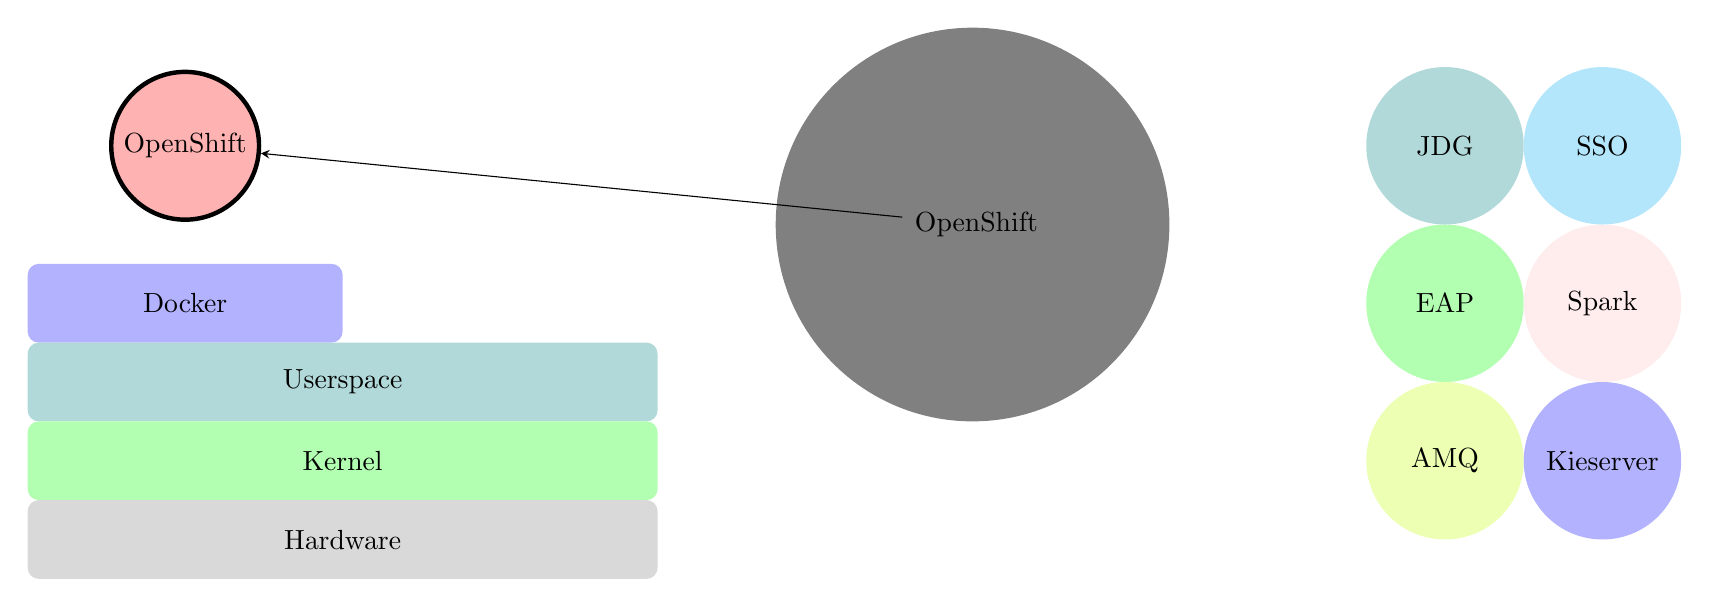
\begin{tikzpicture}[%
    >=stealth,
    node distance=0.05cm,
    on grid,
    auto
  ]
       %Stack
      \tikzstyle{core_stack}=[thick, rounded corners, minimum width=8cm,minimum height=1cm, rectangle]
      \tikzstyle{user_stack}=[ultra thick, rounded corners, minimum width=4cm,minimum height=1cm, rectangle]   
      \draw (-10, 2) node[user_stack, fill=red!30!white, state] (A) {OpenShift}; 
      %\draw (-10, 1) node[user_stack, fill=violet!30!white] {Kubernetes};
      \draw (-10, 0) node[user_stack, fill=blue!30!white] {Docker}; 
      \draw (-8, -1) node[core_stack,  fill=teal!30!white] {Userspace}; 
      \draw (-8, -2) node[core_stack,  fill=green!30!white] {Kernel};
      \draw (-8,-3) node[core_stack,  fill=gray!30!white] {Hardware};  
      
      %OpenShift Bubble
      \fill[black!50!white] (0,1) circle (2.5);
      
    
      %Red Hat Middleware Products
      \fill[lime!30!white] (6,-2) circle (1); %AMQ
      \fill[green!30!white](6,0) circle (1); %EAP
      \fill[teal!30!white] (6,2) circle (1); %JDG
      \fill[blue!30!white] (8,-2) circle (1); %Kieserver
      \fill[pink!30!white] (8,0) circle (1); %Spark
      \fill[cyan!30!white] (8,2) circle (1); %SSO
        %\fill[violet!30!white]  (360:2.5) circle (1); %Tomcat
      \node at (6,-2)    {AMQ};
      \node at (6,0)   {EAP};
      \node at (6,2)   {JDG};
      \node at (8,-2)   {Kieserver};
      \node at (8,0)   {Spark};
      \node at (8,2)   {SSO};
     
      %\node at (360:2.5)    {Tomcat};
      \node (B) [circle, right of=A] at (0,1) {OpenShift}; 
      \%path[->] (B) edge (A);
      \draw [->] (B) edge (A);
    \end{tikzpicture}
\end{figure}
 \fi
%%%%%%%%%%%%%%%%%%%%%%%%%%%%%%%%%%%%%%%%%%%%%%%%%
%%%%%%%%%%%%%%%%%%%%%%%%%%%%%%%%%%%%%%%%%%%%%%%%%

\iffalse
\section{Application Templates}
\indent The CE team generates these container ready applications by using what they call "application-templates". These applications can be generated from premade instructions written in JSON. These templates are the recipes used to cook up the dockerized applications. The application-templates can be found here \url{https://github.com/jboss-openshift/application-templates}

\begin{figure}
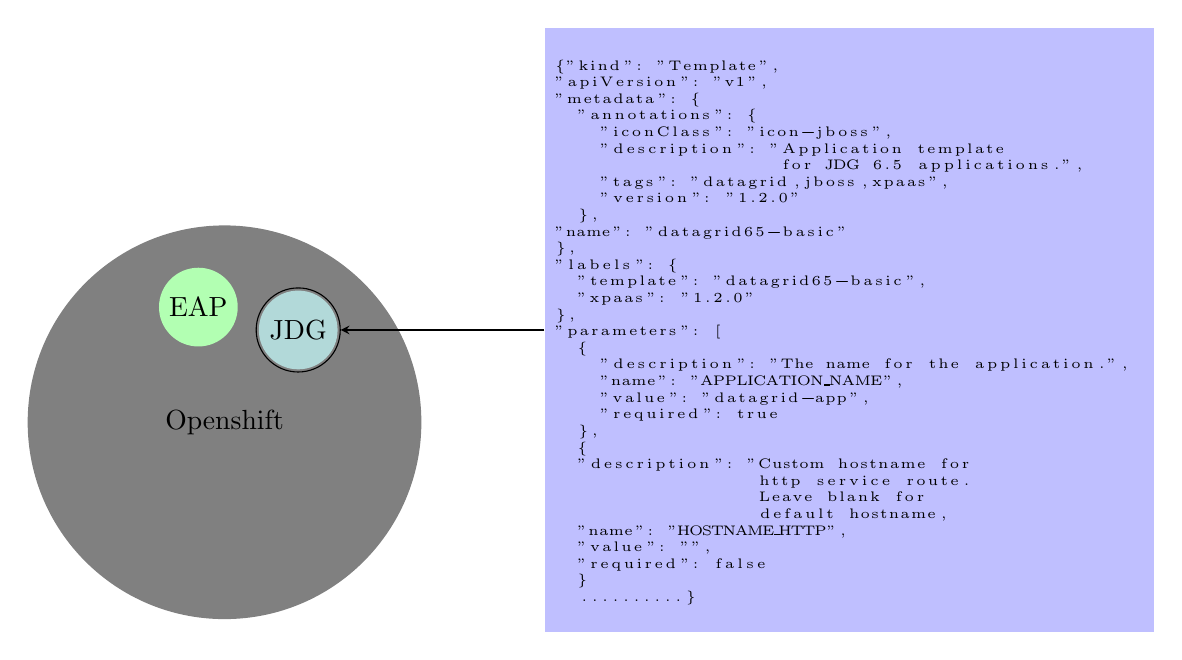
\begin{tikzpicture}[%
    >=stealth,
    node distance=7cm,
    on grid,
    auto
  ]
  \begin{scope}[blend group = soft light]
        %OpenShift Bubble
        \fill[black!50!white]   (0,0) circle (2.5);
  \end{scope}
  \begin{scope}[blend group = soft light]
    \fill[teal!30!white](51.4:1.5) circle (0.5); %JDG
    \fill[green!30!white](102.8:1.5) circle (0.5); %EAP
  \end{scope}
    \node[state] (A) at (51.4:1.5)  {JDG};
    \node at (102.8:1.5) {EAP};
    \node at (0,0)       {Openshift};
    \node (B) [right of=A,fill=blue!25,text width=7.5cm, font=\tiny]{ \begin{lstlisting}
{"kind": "Template",
"apiVersion": "v1",
"metadata": {
  "annotations": {
    "iconClass": "icon-jboss",
    "description": "Application template 
                    for JDG 6.5 applications.",
    "tags": "datagrid,jboss,xpaas",
    "version": "1.2.0"
  },
"name": "datagrid65-basic"
},
"labels": {
  "template": "datagrid65-basic",
  "xpaas": "1.2.0"
},
"parameters": [
  {
    "description": "The name for the application.",
    "name": "APPLICATION_NAME",
    "value": "datagrid-app",
    "required": true
  },
  {
  "description": "Custom hostname for 
                  http service route. 
                  Leave blank for 
                  default hostname,
  "name": "HOSTNAME_HTTP",
  "value": "",
  "required": false
  }
  ..........}
\end{lstlisting}
    };;
    \path[->] (B) edge (A);
  \end{tikzpicture}
\end{figure}
%%%%%%%%%%%%%%%%%%%%%%%%%%%%%%%%%%%%%%%%%%%%%%%%%

\section{Arquillian Components}
  
\begin{lstlisting}
@Test <---- Runs on client
public void testRestService() throws Exception {
  String host = System.getenv("DATAGRID_APP_SERVICE_HOST");
  int port = Integer.parseInt(System.getenv("DATAGRID_APP_SERVICE_PORT"));
  RESTCache<String, Object> cache = new RESTCache<>("default", new URL("http://" + host + ":" + port), "rest");
  cache.put("foo1", "bar1");
  assertEquals("bar1", cache.get("foo1"));
}
\end{lstlisting}


\begin{lstlisting}
|@Test|   
|@RunAsClient|
|@InSequence(1)|
public void testCarMartApp() throws Exception {
  Car car = new Car("test", 0.0, CarType.SEDAN, "test", "test", Country.USA);
  client = HttpClientBuilder.untrustedConnectionClient();
  addCar(car);
	assertCarsAreSame(car, getCar(car));
}
\end{lstlisting}

\noindent Before we dive into the details of the testsuite, we must first understand the Arquillian components. When maven builds an application, it spawns two JVMs; one for the testrunner and one for the tests. Take the following example for example

\begin{lstlisting}[style=Java]
|@Test|    <-------------- Local Test
|@RunAsClient|
|@InSequence(1)|
public void testCarMartApp() throws Exception {
  Car car = new Car("test", 0.0, CarType.SEDAN, "test", "test", Country.USA);
  client = HttpClientBuilder.untrustedConnectionClient();
  addCar(car);
	assertCarsAreSame(car, getCar(car));
}
\end{lstlisting}


\begin{lstlisting}
|@RunWith|(Arquillian.class)
|@Template|(url="https://raw.githubusercontent.com/jboss-openshift/application-templates/master/datagrid/datagrid65-basic.json")
|@RoleBinding|(roleRefName = "view", userName = "system:serviceaccount:\${kubernetes.namespace}:jdg-service-account")
|@OpenShiftResources|({
  |@OpenShiftResource|("https://raw.githubusercontent.com/\${template.repository:jboss-openshift}/application-templates/\${template.branch:master}/secrets/datagrid-app-secret.json")
})
public class JdgBasicTest extends JdgTestBase {
  |@Deployment|
  public static WebArchive getDeployment() {
    return getDeploymentInternal();
  }
}
\end{lstlisting}

  %\begin{scope}[blend group = soft light] 
        %\fill[lime!30!white] (51.4:2.5) circle (1); %AMQ
        %\fill[green!30!white] (102.8:2.5) circle (1); %EAP
        %\fill[teal!30!white]  (154.2:2.5) circle (1); %JDG
        %\fill[blue!30!white]  (205.7:2.5) circle (1); %Kieserver
        %\fill[pink!30!white]  (257.1:2.5) circle (1); %Spark
        %\fill[cyan!30!white]  (308.5:2.5) circle (1); %SSO
        %\fill[violet!30!white]  (360:2.5) circle (1); %Tomcat
      %\end{scope}
      %\node at (51.4:2.5)    {AMQ};
      %\node at (102.8:2.5)   {EAP};
      %\node at (154.2:2.5)   {JDG};
      %\node at (205.7:2.5)   {Kieserver};
      %\node at (257.1:2.5)   {Spark};
      %\node at (308.5:2.5)   {SSO};
      %\node at (360:2.5)    {Tomcat};
\fi
\end{document}
